\chapter{Appendix - Model parameters for trajectory match}

\begin{figure}[!htb]
  \subfloat[Far-field matching\label{Appendix-1}]{
    
\includegraphics[totalheight=5cm,trim={0 0 0 0},clip]{parameter_match_3.eps}
  }
  \hfill
  \subfloat[Quadrupolar moment\label{Appendix-2}]{
    
\includegraphics[totalheight=5cm,trim={0 0 0 0},clip]{parameter_match_4.eps}
  }
  \\
  \subfloat[Near field matching\label{Appendix-3}]{
    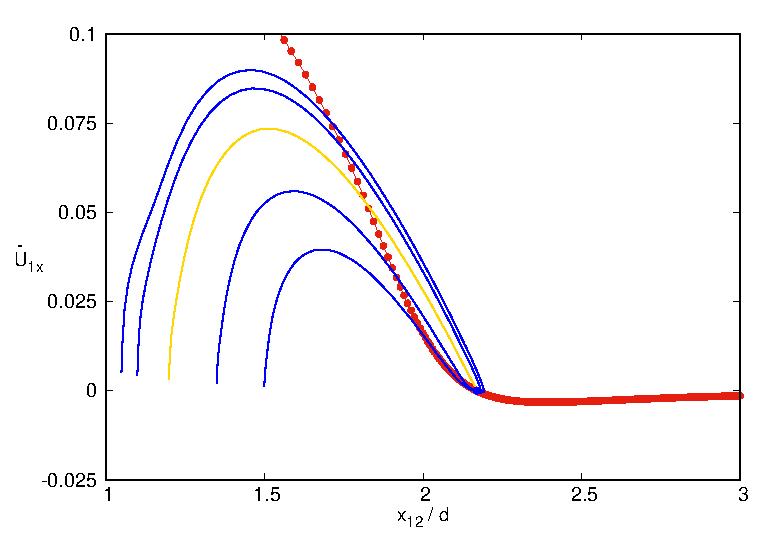
\includegraphics[totalheight=5cm,trim={0 0 0 0},clip]{parameter_match_1_after_z_introduction_zshift.eps}
  }
  \hfill
  \subfloat[Deformation induced velocity\label{Appendix-4}]{
    
\includegraphics[totalheight=5cm,trim={0 0 0 0},clip]{gradient_vel-gradient_pos.eps}
  }
  \caption{~\ref{Appendix-1} show particle trajectories for long inital separation from FD/FT simulations and the corresponding matching with the velocity $\mathbf{U}_{xi}$ form the Hele--Shaw model. ~\ref{Appendix-2} show the ratio of far-field velocity from FD/FT simulations and quadrupolar velocity from the model simulations. ~\ref{Appendix-3} shows particle trajectories for a range on initial separations $x_{12}^{(0)}/d = $ 1.05, 1.1, 1.2, 1.35, 1.5 from FD/FT simulations and matching. ~\ref{Appendix-4} show the deformation induced velocity, along gradient direction, versus the particle position along the same.}
  \label{Appendix}    
  
\end{figure}

Here the evaluation of the parameters introduced in Chapter~\ref{phenomenon} are discussed. A unit cell of dimensions $23d\times 4d$, in the flow and vorticity directions respectively, was used to run the simulation between particle pair. In our 3-D model too, simulations were performed in a cell of exact same dimensions. The quadrupolar interactions are calculated in a periodic manner by the usage of Ewald-sum and the swapping-trajectory effect has been calculated using direct-summation.

First, two particles were place along the flow direction with an initial separation of $x_{12}^{(0)}/d = 4$ in the mid-plane of the channel. Fig.~\ref{Appendix-1} shows the long-range  particle trajectories and Fig.~\ref{Appendix-2} shows the ratio of the the relative velocities of the particles obtained from the direct numerical simulations and the 3-D model. We observe that the attractive velocity reaches a maxima at $x_{12}/d \approx 2.4$ and thereafter keeps decreasing andfinally the particles stop and stagnate at $x_{12}/d \approx 2.17$ which is essentially the stopping distance($l_{st}$) of a the particles. Therefore in the range of $x_{12}[2.4:4]$ it can be concluded that the system evolution is controlled by both the quadrupolar and swapping-trajectory interactions.

Second, we introduce a particle pair at a range of separations $x_{12}^{(0)}/d = $ 1.05, 1.1, 1.2, 1.35, 1.5 to study the short range relative motion and thereby extract the remaining parameters. Fig~\ref{Appendix-3} shows the short-range trajectories of particles. To obtain the prameters of the swapping-trajectory model in the flow-driection, we obtain such values of the parameters that would qualitatively match all of the trajectories with the intention of replicating the key features in the 3-D model.
Finally, Fig.~\ref{Appendix-4} the gradient direction velocity with respect to the gradient direction position of an individual particle suspended at $z_{1}/d = 1.28$ away from the mid-plane. The particle initially deforms and then starts its migration towards the z=1.2(in our case z=0) plane. This illustrates the fact that the deformation induced velocity in confined channels under shear-flow for small distances is linearly proportional to the gradient direciton position.